\subsection*{Problem 1}
Decide if there exists a graph with the following degree sequence: 
\[
1,1,1,2,4,5,6,6,7
\]


\begin{solution}
There does not exist such a graph. The sum of the degrees of a graph's vertices must be even ($2|E|$), but here, the sum of the degrees is 33, which is odd.
\end{solution}

\subsection*{Problem 2}
Prove that any simple graph on at least 2 vertices contains two vertices having the same degree.

\begin{proof}
Suppose a simple graph $G = (V,E)$ has $n \geq 2$ vertices. Then for any $v \in V$, $d(v) \leq n-1$ and $d(v) \in \{ 0,\dots,n-1 \}$. Since we have $n$ vertices and $n-1$ degree ``options'', at least two vertices must fall in the same degree ``option''. Note that if $d(v)=0$ for some $v \in V$, then you cannot have another vertex $v' \in V$ with $d(v')=n-1$. Thus, there are at least two vertices having the same degree.
\end{proof}

\subsection*{Problem 3}
Verify that for any graph $G=(V,E)$, either $G$ or its compliment $\overline{G}$ is connected.

\begin{proof}
If $G$ is connected, then we are done. Otherwise, if $G$ is not connected, then there exist vertices $u,v \in V$ such that there is no path from $u$ to $v$. This implies that there are two subgraphs $A = (V_A, E_A)$ and $B = (V_B, E_B)$ of the graph $G = (V, E)$ such that $ V_A \cap V_B = \emptyset $ and $ V_A \cup V_B = V $ and for every $a \in V_A$ and $b \in V_B$, $ab \notin E$. Now, in the compliment $\overline{G} = (\overline{V}, \overline{E})$, for every $a \in V_A$ and $b \in V_B$, $ab \in \overline{E}$. Thus there exists paths between any vertex in $V_A$ and any vertex in $V_B$, and any vertices $u,v \in V_B$ has a path via a vertex in $V_A$ and any vertices $u,v \in V_A$ has a path via a vertex in $V_B$. So $\overline{G}$ is connected.
\end{proof}

\subsection*{Problem 4}
Prove that if $G=(V,E)$ is a simple graph on $2n$ vertices such that every vertex has degree at least $n$, then $G$ is connected.

\begin{proof}
We will proceed inductively. For the base case, assume $n=1$. A graph with 2 vertices with a connection between them is connected. Assume a simple graph on $2n$ vertices such that every vertex has degree at least $n > 1$ is connected. We will prove that a graph on $2(n+1)=2n+2$ vertices such that every vertex has at least degree $n+1$ is connected as well. We are taking the connected graph with $2n$ vertices and adding 2 additional vertices. We are also then taking each vertex and adding 1 to it's degree, effectively adding an edge that it previously did not have. Note that these 2 new vertices can either connect to itself, or connect to a vertex that exists within this connected section. Since these vertices each has degree at least $n+1$, each of them must connect back to the connected path of the graph. Thus, this newly constructed graph is connected as well.
\end{proof}

\subsection*{Problem 5}
Prove that any connected graph has a vertex whose deletion (together with the edges incident to it) results in a connected graph.

\begin{proof}
We know that the vertices of a connected graph $G$ can always be enumerated as $v_1, \dots, v_n$ so that 
$G_i := G[v_1, \dots, v_i]$ is connected for every $i$. Setting $i = n$, we have $G_n = G[v_1, \dots, v_n]$. Consider the vertex $v_n$. Deleting it results in the graph $G_{n-1} = G[v_1, \dots, v_{n-1}]$ which is still connected.
\end{proof}

\subsection*{Problem 6}
Prove that if $G=(V,E)$ is a graph with at least 5 vertices, then either $G$ or $\overline{G}$ contains a cycle.

\begin{proof}
If $G$ contains a cycle, then we are done. Otherwise, let $G$ be an n vertex graph without a cycle with $n>5$. Then $G$ is a forest with $1 \leq d \leq 5$ trees. 
We know then that the number of edges $|E_G| \leq n-1$. In $\overline{G}$, however, we have $|E_{\overline{G}}| = |E_{K_n}|-|E_G|= \frac{n(n-1)}{2} - |E_G| \geq \frac{n(n-1)}{2} + n - 1$ \footnote{We know $|E_{K_n}| = \frac{n(n-1)}{2}$ because given $n$ vertices, we first connect one of them to the other $n-1$ vertices, then another one to the remaining $n-2$ vertices and so on. In the end we have the sum $\sum_{1}^{n-1} = \frac{n(n-1)}{2} $.}.
Note then that for all $n>5$, $|E_{\overline{G}}| \geq \frac{n(n-1)}{2} + n - 1 > n - 1$. Since this compliment graph has greater than $n-1$ edges, it has more edges that it's spanning tree, and thus is no longer a tree and contains a cycle.
\end{proof}


\subsection*{Problem 7}
Determine the tree whose Prüfer code is $(4,4,7,4,1)$.

\begin{solution}
\begin{center}
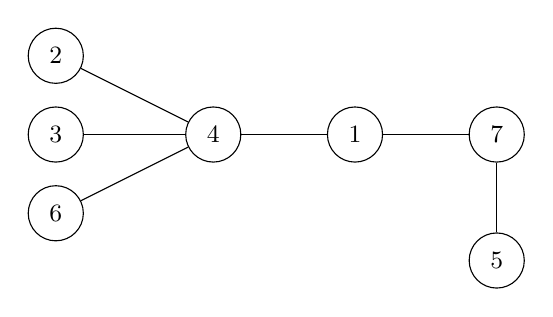
\begin{tikzpicture}[every node/.style={circle,draw,minimum size=7mm,font=\small}]
  \node (4) at (0,0) {4};
  \node (2) at (-2,1) {2};
  \node (3) at (-2,0) {3};
  \node (6) at (-2,-1) {6};
  \node (1) at (1.8,0) {1};
  \node (7) at (3.6,0) {7};
  \node (5) at (3.6,-1.6) {5};

  \draw (4)--(2);
  \draw (4)--(3);
  \draw (4)--(6);
  \draw (4)--(1);
  \draw (1)--(7);
  \draw (7)--(5);
\end{tikzpicture}
\end{center}
\end{solution}

\subsection*{Problem 8}
Characterize those trees whose Prüfer code consists of all different numbers.

\begin{solution}
If a tree with length $n$ has a Prüfer code has no repeating number, then the tree is just a straight path with length $n$. The code has length $n-2$. In the tree, there are 2 vertices with degree 1, and they don't appear in the code. The other $n-2$ vertices each appear once in the code, which means they have degree 2, and these are the inner vertices of the path. 
\end{solution}

\subsection*{Problem 9}
Let $T$ be a tree whose Prüfer code consists of the same number. What is the maximum length of a path in $T$?

\begin{solution}
If the Prüfer code of $T$ consists of the same number, then there is exactly one vertex (whose label is the only number in the Prüfer code) with many leaves. So the maximum length of a path in $T$ is 2, with this maximal path going from a leaf to the main node to another leaf.
\end{solution}

\subsection*{Problem 10}
Determine the number of trees on vertices $1, \ldots, n$ in which vertex 1 has degree exactly 2.

\begin{solution}
We can count the number of Prüfer codes (with length $n-2$) that represent this tree. Since vertex 1 has degree exactly 2, it appears exactly once in the code, and there are $n-2$ choices where it can go. We then have have $n-1$ other labels with $n-3$ positions where they can go. Thus, we have $(n-2)(n-1)^{n-3}$ such trees.
\end{solution}